    %%%%%%%%%%%%%%%%%%%%%%%%%%%%%%%%%%%%%%%%%%%%%%%%%%%%%%%%%%%%%%%%%%%%%%
% How to use writeLaTeX: 
%
% You edit the source code here on the left, and the preview on the
% right shows you the result within a few seconds.
%
% Bookmark this page and share the URL with your co-authors. They can
% edit at the same time!
%
% You can upload figures, bibliographies, custom classes and
% styles using the files menu.
%
% If you're new to LaTeX, the wikibook is a great place to start:
% http://en.wikibooks.org/wiki/LaTeX
%
%%%%%%%%%%%%%%%%%%%%%%%%%%%%%%%%%%%%%%%%%%%%%%%%%%%%%https://v2.overleaf.com/project/5baac094de0904180e28e9b3%%%%%%%%%%%%%%%%%
\documentclass{tufte-handout}

%\geometry{showframe}% for debugging purposes -- displays the margins

\usepackage{amsmath}

% Set up the images/graphics package
\usepackage{graphicx}
\setkeys{Gin}{width=\linewidth,totalheight=\textheight,keepaspectratio}
\graphicspath{{graphics/}}

\title{How Factor Drive\texttrademark Works}
\author[Hugh Winkler]{Hugh Winkler}
\date{23 October 2018}  % if the \date{} command is left out, the current date will be used

% The following package makes prettier tables.  We're all about the bling!
\usepackage{booktabs}

% The units package provides nice, non-stacked fractions and better spacing
% for units.
\usepackage{units}

% The fancyvrb package lets us customize the formatting of verbatim
% environments.  We use a slightly smaller font.
\usepackage{fancyvrb}
\fvset{fontsize=\normalsize}

% Small sections of multiple columns
\usepackage{multicol}

% Provides paragraphs of dummy text
\usepackage{lipsum}

% These commands are used to pretty-print LaTeX commands
\newcommand{\doccmd}[1]{\texttt{\textbackslash#1}}% command name -- adds backslash automatically
\newcommand{\docopt}[1]{\ensuremath{\langle}\textrm{\textit{#1}}\ensuremath{\rangle}}% optional command argument
\newcommand{\docarg}[1]{\textrm{\textit{#1}}}% (required) command argument
\newenvironment{docspec}{\begin{quote}\noindent}{\end{quote}}% command specification environment
\newcommand{\docenv}[1]{\textsf{#1}}% environment name
\newcommand{\docpkg}[1]{\texttt{#1}}% package name
\newcommand{\doccls}[1]{\texttt{#1}}% document class name
\newcommand{\docclsopt}[1]{\texttt{#1}}% document class option name

\begin{document}

\maketitle% this prints the handout title, author, and date

\begin{abstract}
\noindent
Factor Drive\texttrademark solves the geosteering problem probabilistically.
It models everything in the system as random variables, and then  
calculate the probability of each possible configuration of those variables.
\end{abstract}

%\printclassoptions



\section{How It Doesn't Work}\label{sec:how-it-doesnt-work}
Let's dispose of a misleading idea. 
Factor Drive\texttrademark doesn't simulate the way people use a conventional geosteering program.
It doesn't try a lot of different geologic structures and wellbore trajectories, selecting
the configuration that gives the best correlation between the type log and the MWD gamma ray. The
interpretation that gives the best
correlation may not be the most likely one.
Correlation is a good guide. Under many common circumstances it does give you the best
interpretation. But the assumptions it requires aren't broad enough to support using
it to compute an interpretation.
Correlation can fail if there are ambiguous, nearly identical features on the log; a fault can cause a misleading alignment. Mathematically, we'd say that the "best correlation" rule fails because the variables you're optimizing aren't normally distributed.

Geologists know how to work around these limitations. They overrule the numbers whenever geologic or engineering sense dictates. Factor Drive\texttrademark captures those heuristics as probability distributions.

\section{How It Works}\label{sec:how-it-doesnt-work}
\subsection{The Fundamental Problem of Geosteering}\label{sec:fundamental-problem}

\begin{marginfigure}
  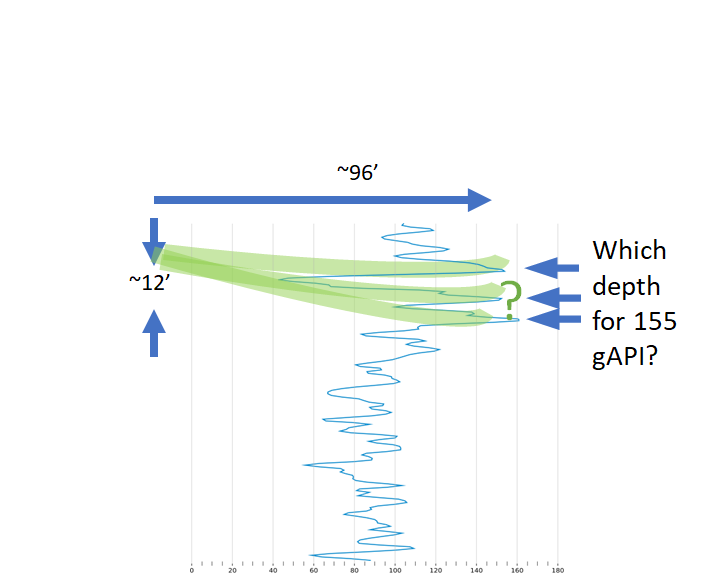
\includegraphics{which-depth-for-155-gapi.png}
  \caption{This gamma ray type log touches near 155 gAPI at three separate depths.}
  \label{fig:which-depth-for-155-gapi}
\end{marginfigure}

The fundamental problem of geosteering is: given a log reading while drilling, what stratigraphic depth did it come from?

If you only knew that a GR reading of 155 gAPI came from somewhere in the depth range on figure
\ref{fig:which-depth-for-155-gapi}, you'd know that the reading probably came from one of the three depths where the log reaches that value. By "probably", we mean we can represent that knowledge by a
probability distribution, as in figure \ref{fig:probability-density-for-155-gapi}. 






Just consider a few positions along a lateral wellbore, as in figure~\ref{fig:random-vars-lateral} . We'll work in
two dimensions, to make life easy. At each position,
think of these quantities as random variables: the spatial location
of the position, and the depth of the geologic structure at that position's lateral location.
These are the quantities we want to know. Since they are random variables, we'll describe the
answers as probability distributions. 


\begin{marginfigure}
  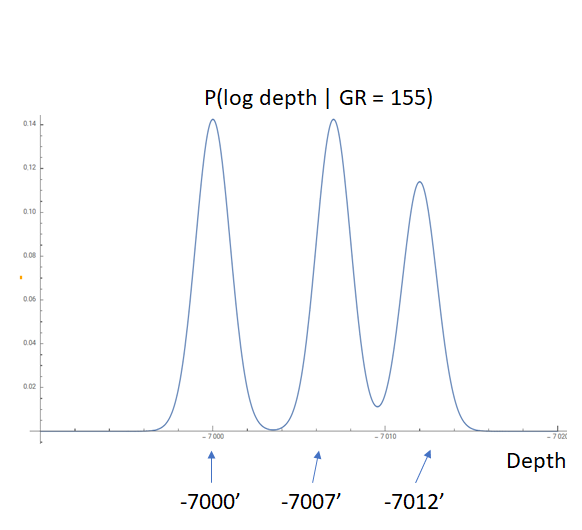
\includegraphics{probability-density-for-155-gapi.png}
  \caption{The probability that a log reading of 155 gAPI came from any particular depth.}
  \label{fig:probability-density-for-155-gapi}
\end{marginfigure}



So to visualize the computed probability for the wellbore position's spatial location,
imagine a hill rising out of the (depth, lateral) plane. The peak of the hill occurs at the
most likely value of the wellbore's spatial location, but the other points on the plane where
the hill has appreciable height could also be the true values.To visualize the computed
probability for the depth of the structure at that position's lateral location, you could
just imagine a 1-D "hill", or distribution over depth. And sometimes, the answers might show
two hills for a random variable; there can be more than one likely answer.

\begin{marginfigure}
  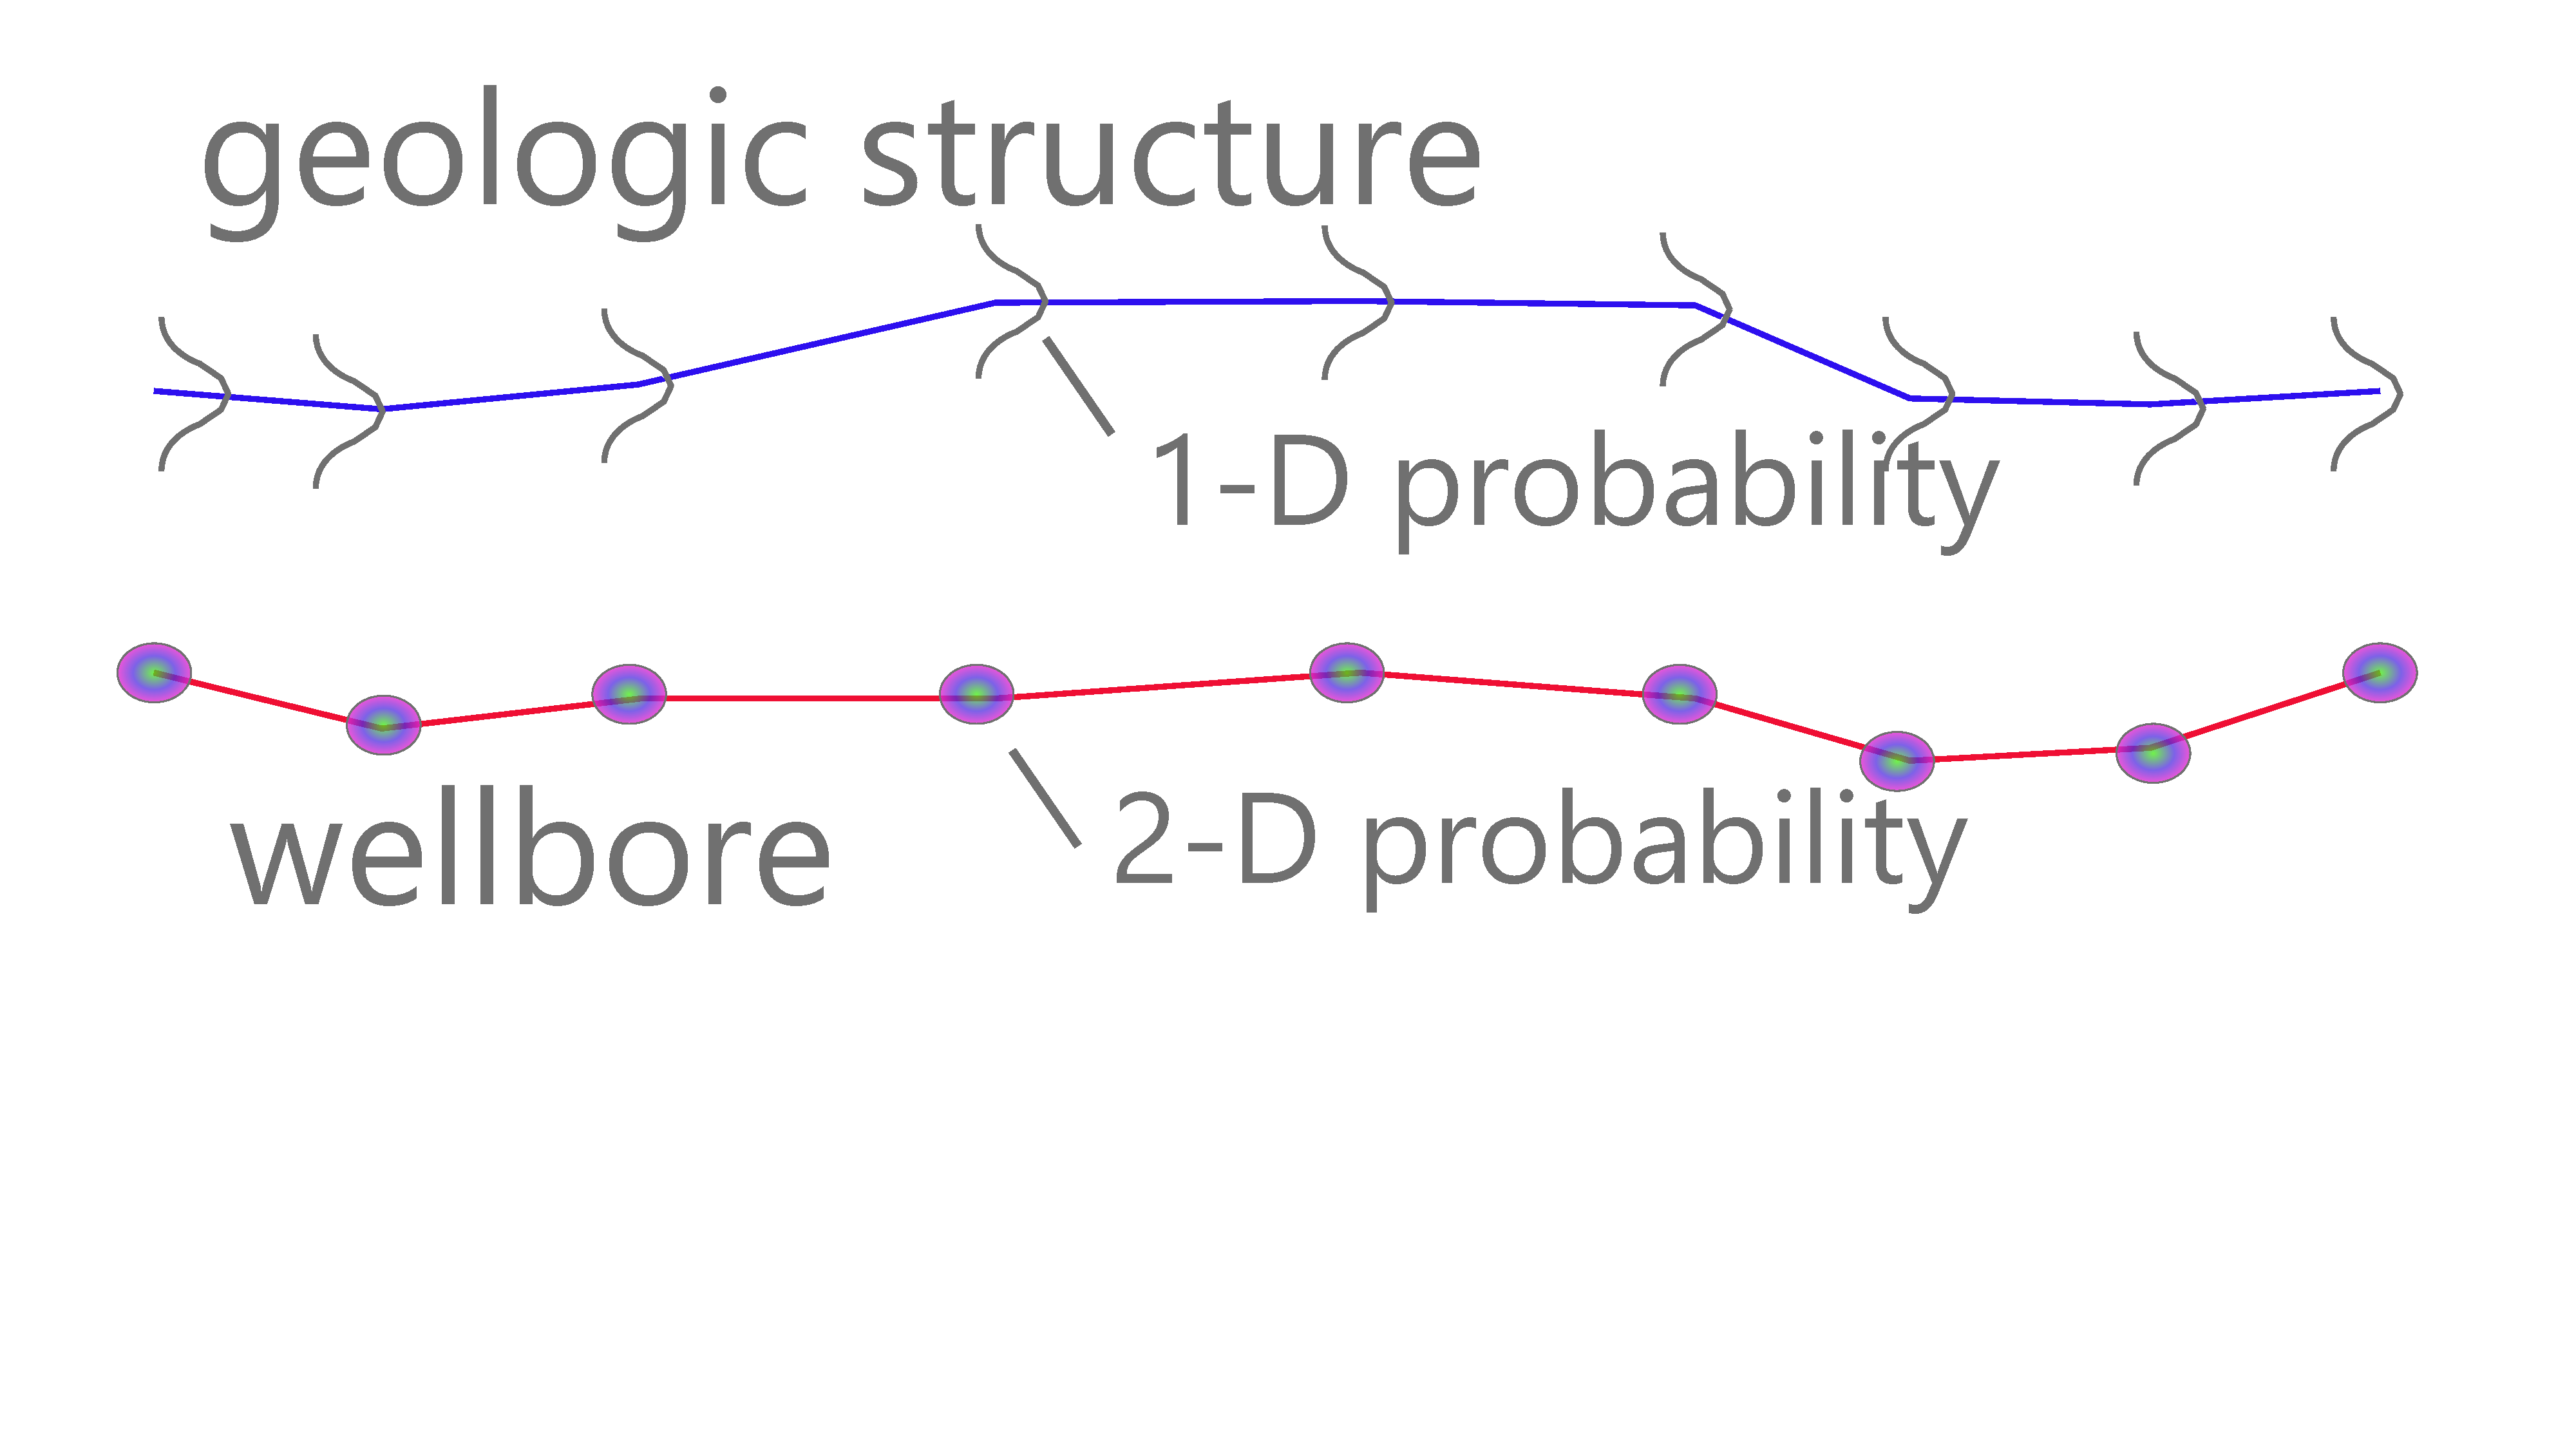
\includegraphics{random-vars-lateral}
  \caption{Think of the wellbore as a series of points having 
  uncertain locations, and of the geologic structure as a series
  of points located laterally with those wellbore positions, having uncertain depths. In this figure I've rendered 18 random variables: nine for the well locations, and nine for the geologic structure depths. The wellbore locations have uncertainty in the lateral as well as the depth dimension; the structure depths have uncertainty only in the depth dimension. Think of these uncertainties as probability distributions.}
  \label{fig:random-vars-lateral}
\end{marginfigure}

So that's how we represent the answers, but what about the measurements? We also represent those as probability distributions. 


\begin{marginfigure}
  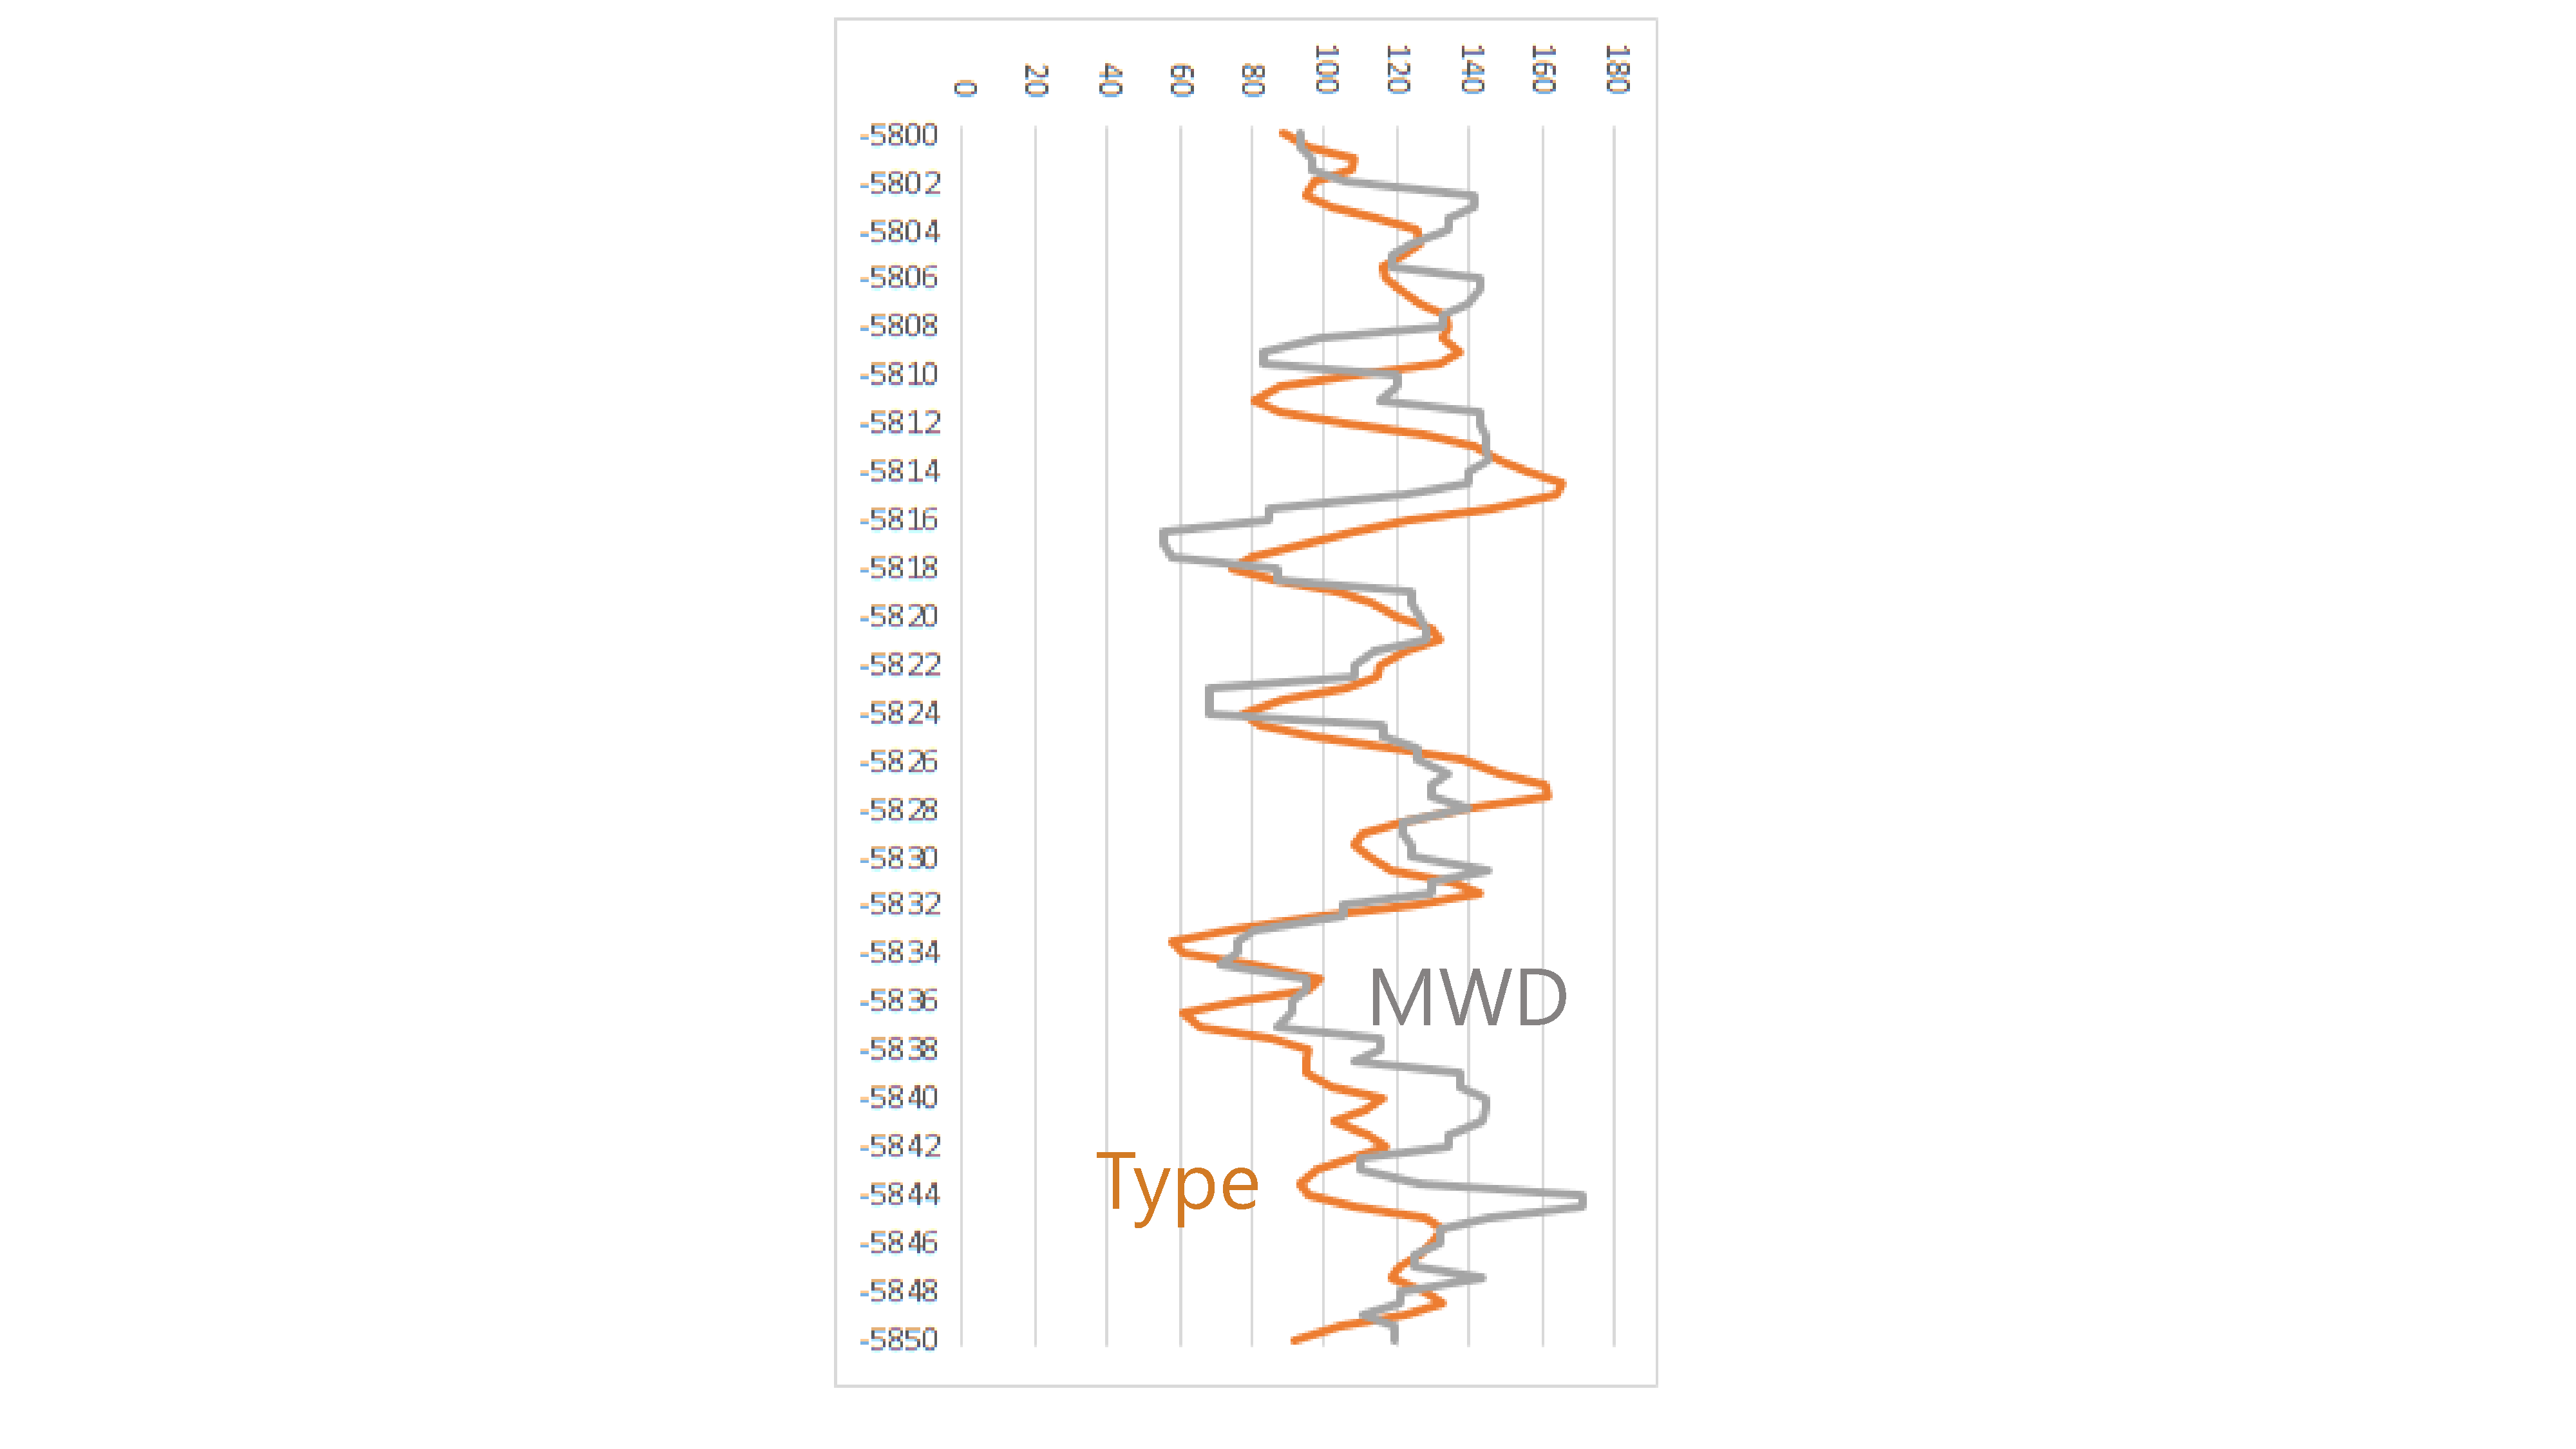
\includegraphics{logfit}
  \caption{A type log and the MWD over a fifty foot depth range}
  \label{fig:logfit}
\end{marginfigure}


Given a depth value, the type log tells you the GR value there.  The fundamental problem of geosteering is: Given a GR value, tell us its depth on the type log. That inverse mapping is usually ambiguous. Many depths on the type log may have the same GR value. On the colored type log curve in  figure \ref{fig:logfit}, the log cuts through 140 gAPI at several depths. If you read 140 gAPI on the MWD, which of these depths is the hole exploring? 

Figure \ref{fig:gr-depth-histogram} is a very coarse, 2-D histogram counting the occurences of depth.
You can
If you take a slice through that figure for GR = 140, you get a probability distribution (figure \ref{fig:gr140-histogram}) 
for the likely depth on the log


\begin{marginfigure}
  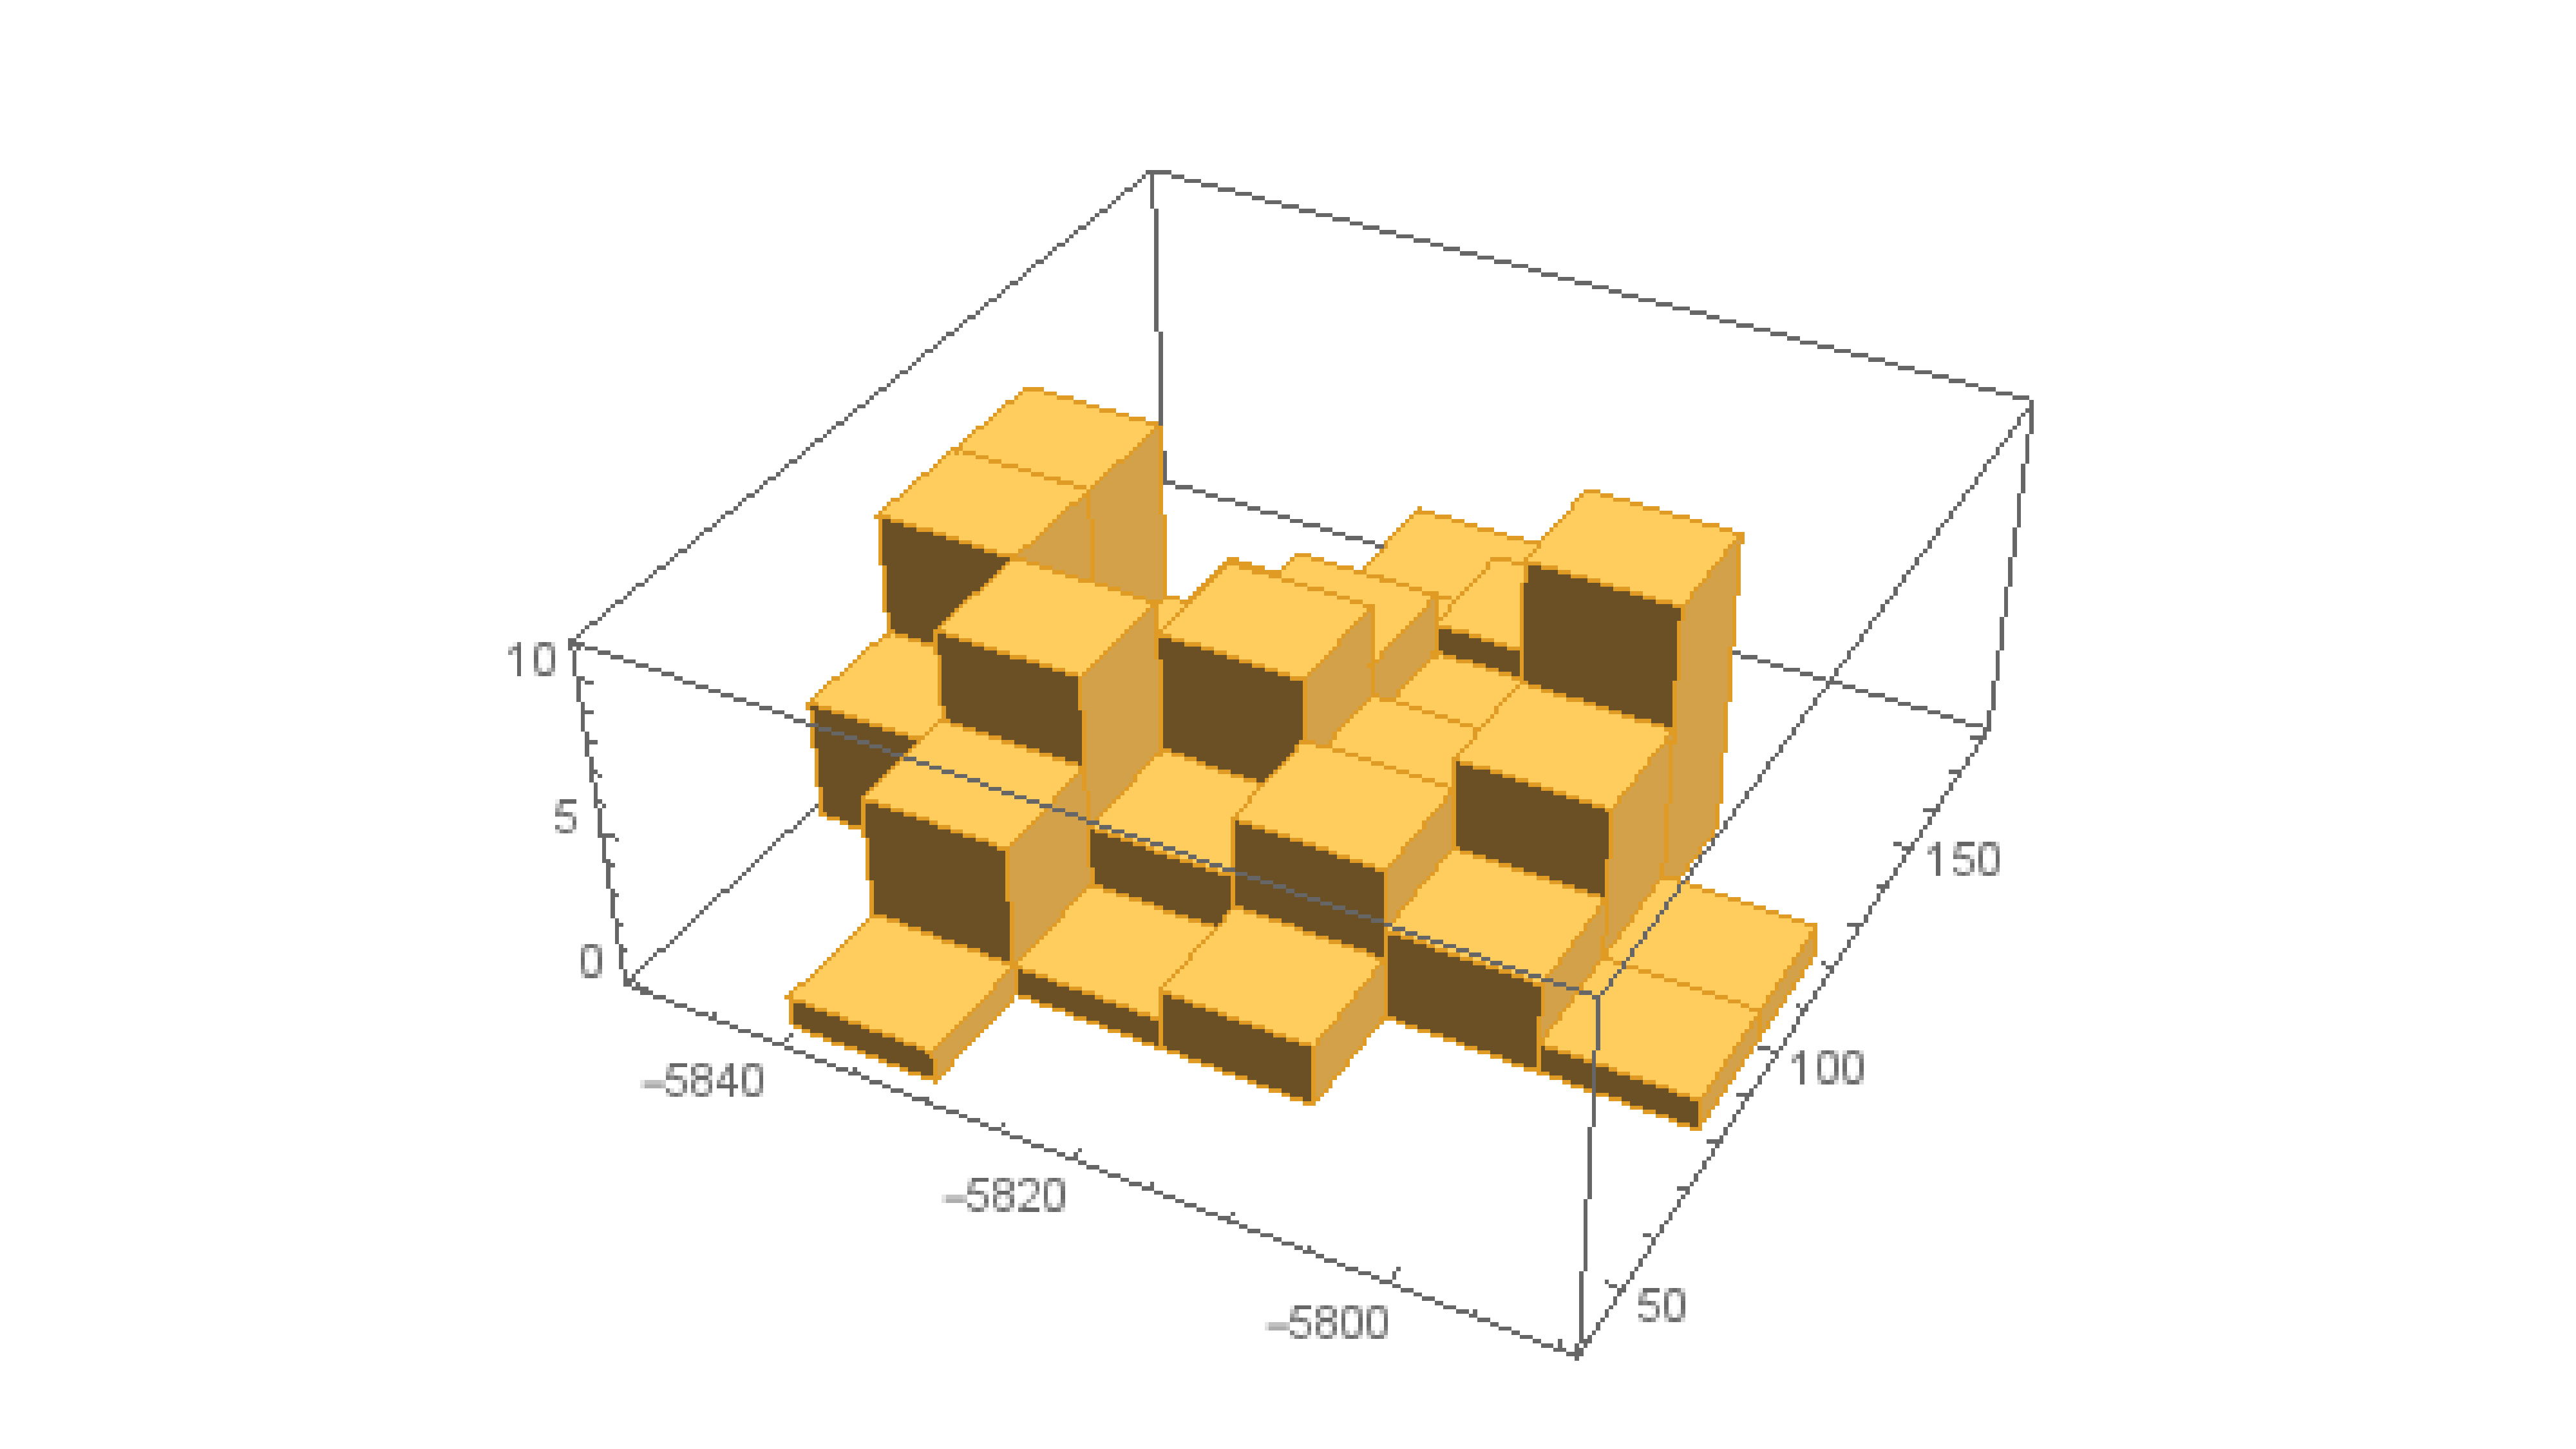
\includegraphics{gr-depth-histogram}
  \caption{I made this histogram over the samples from 50 feet of 
  a type log. One axis is depth; the other is GR log value.
  Given a GR log value in the MWD, there are multiple possible depths
  that could explain it. }
  \label{fig:gr-depth-histogram}
\end{marginfigure}


Survey instruments have well documented error models. Directional companies remove all the persistent errors, such as errors due to magnetized wellbore components, or geodetic errors. The remaining uncertainty is usually a simple normal distribution around the inclination reading, like a bell curve. That error can sometimes spread out as much a one degree above or below the measured value. 

\begin{marginfigure}
  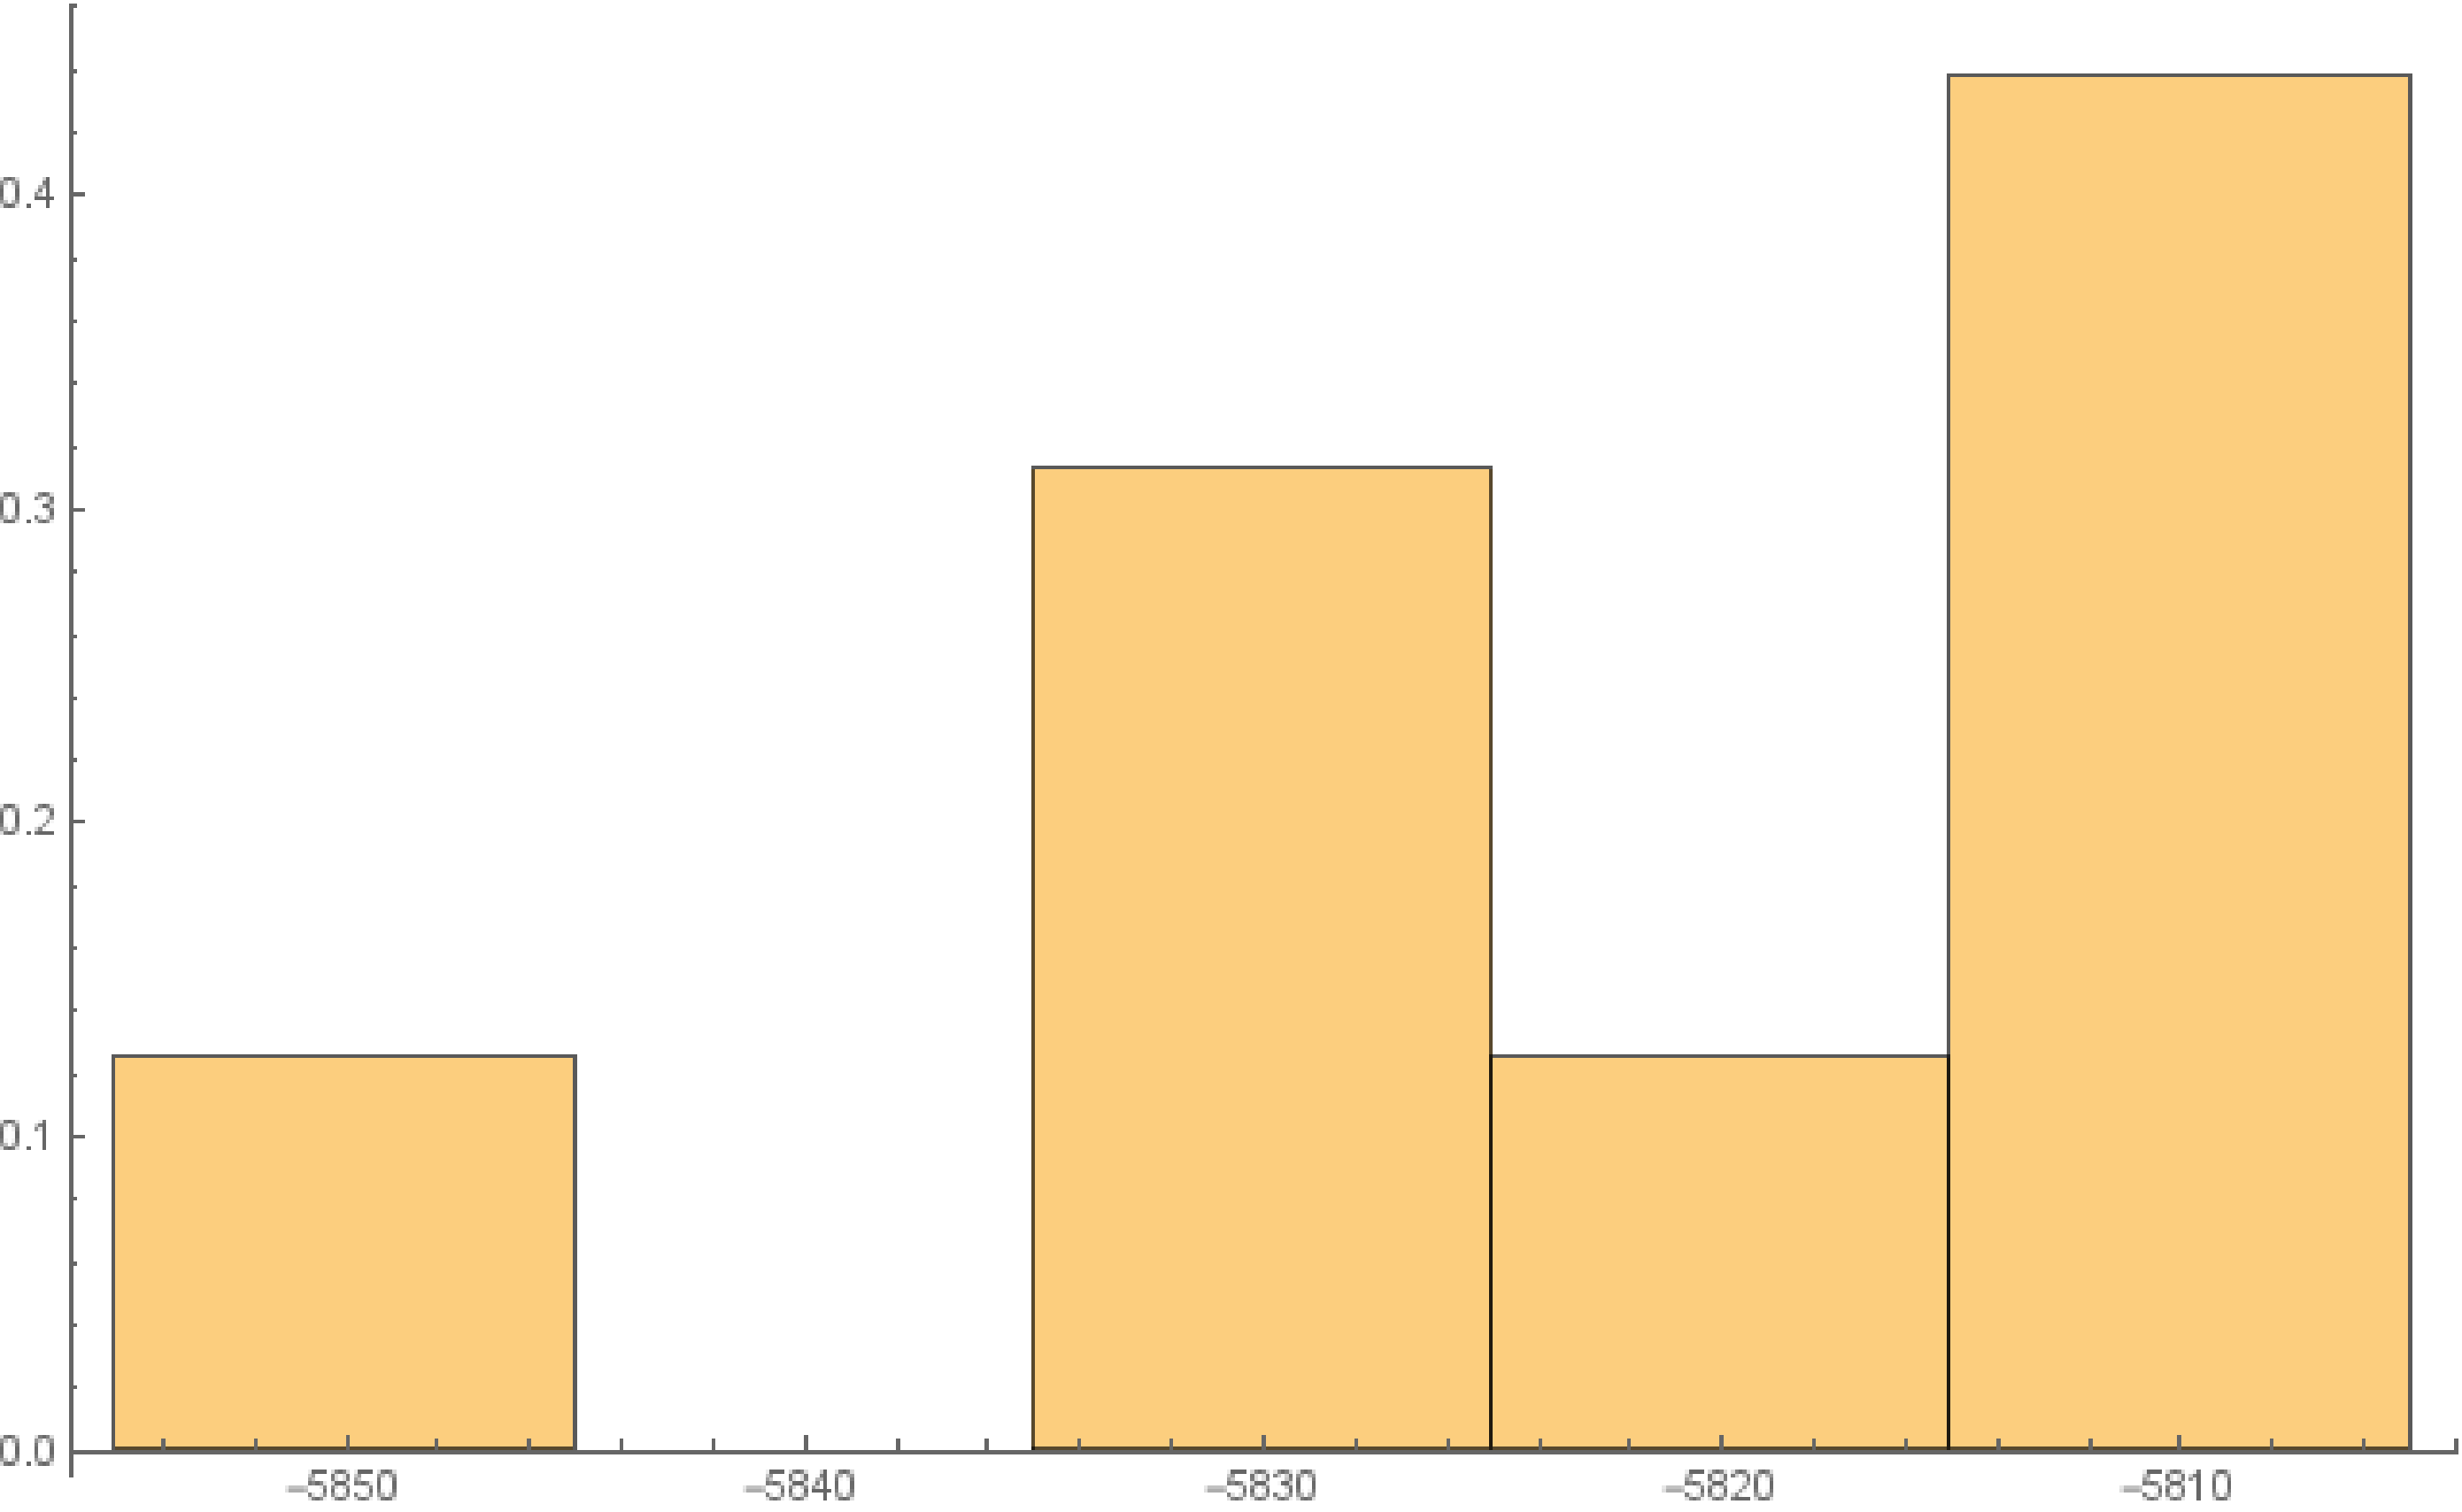
\includegraphics{gr140-histogram}
  \caption{If we see a GR value of 140, and all we know is that we're in the
  depth range -5850 to -5000, this histogram (coarsely) represents our probability
  of being at }
  \label{fig:gr140-histogram}
\end{marginfigure}

Gamma ray log values, by their nature, are statistical. Even using the same instrument, logging the same section of hole repeatedly gives slightly different results. But in our model, it's more relevant to think about the statistical differences between the MWD gamma ray and the type log. After you've fitted the log from some pilot well to the MWD GR, scaling and shifting it so that it looks as much as possible like the MWD you're acquiring, there remain differences between the two logs. Generally, those differences obey a Laplace distribution; see figure \ref{fig:log-histogram}.
By these statistics, we anticipate that when you read an MWD value in this well -- say, 90 gAPI -- you probably are in a stratum on the type log that also has a 90 gAPI background gamma. But it \emph{might} have come from a stratum that normally reads 40 gAPI, and for various reasons (tool temperature, tool speed of travel, eccentering in hole, or rock that has a random but local variation) this particular time reads a 50 gAPI difference from usual. 


\begin{marginfigure}
  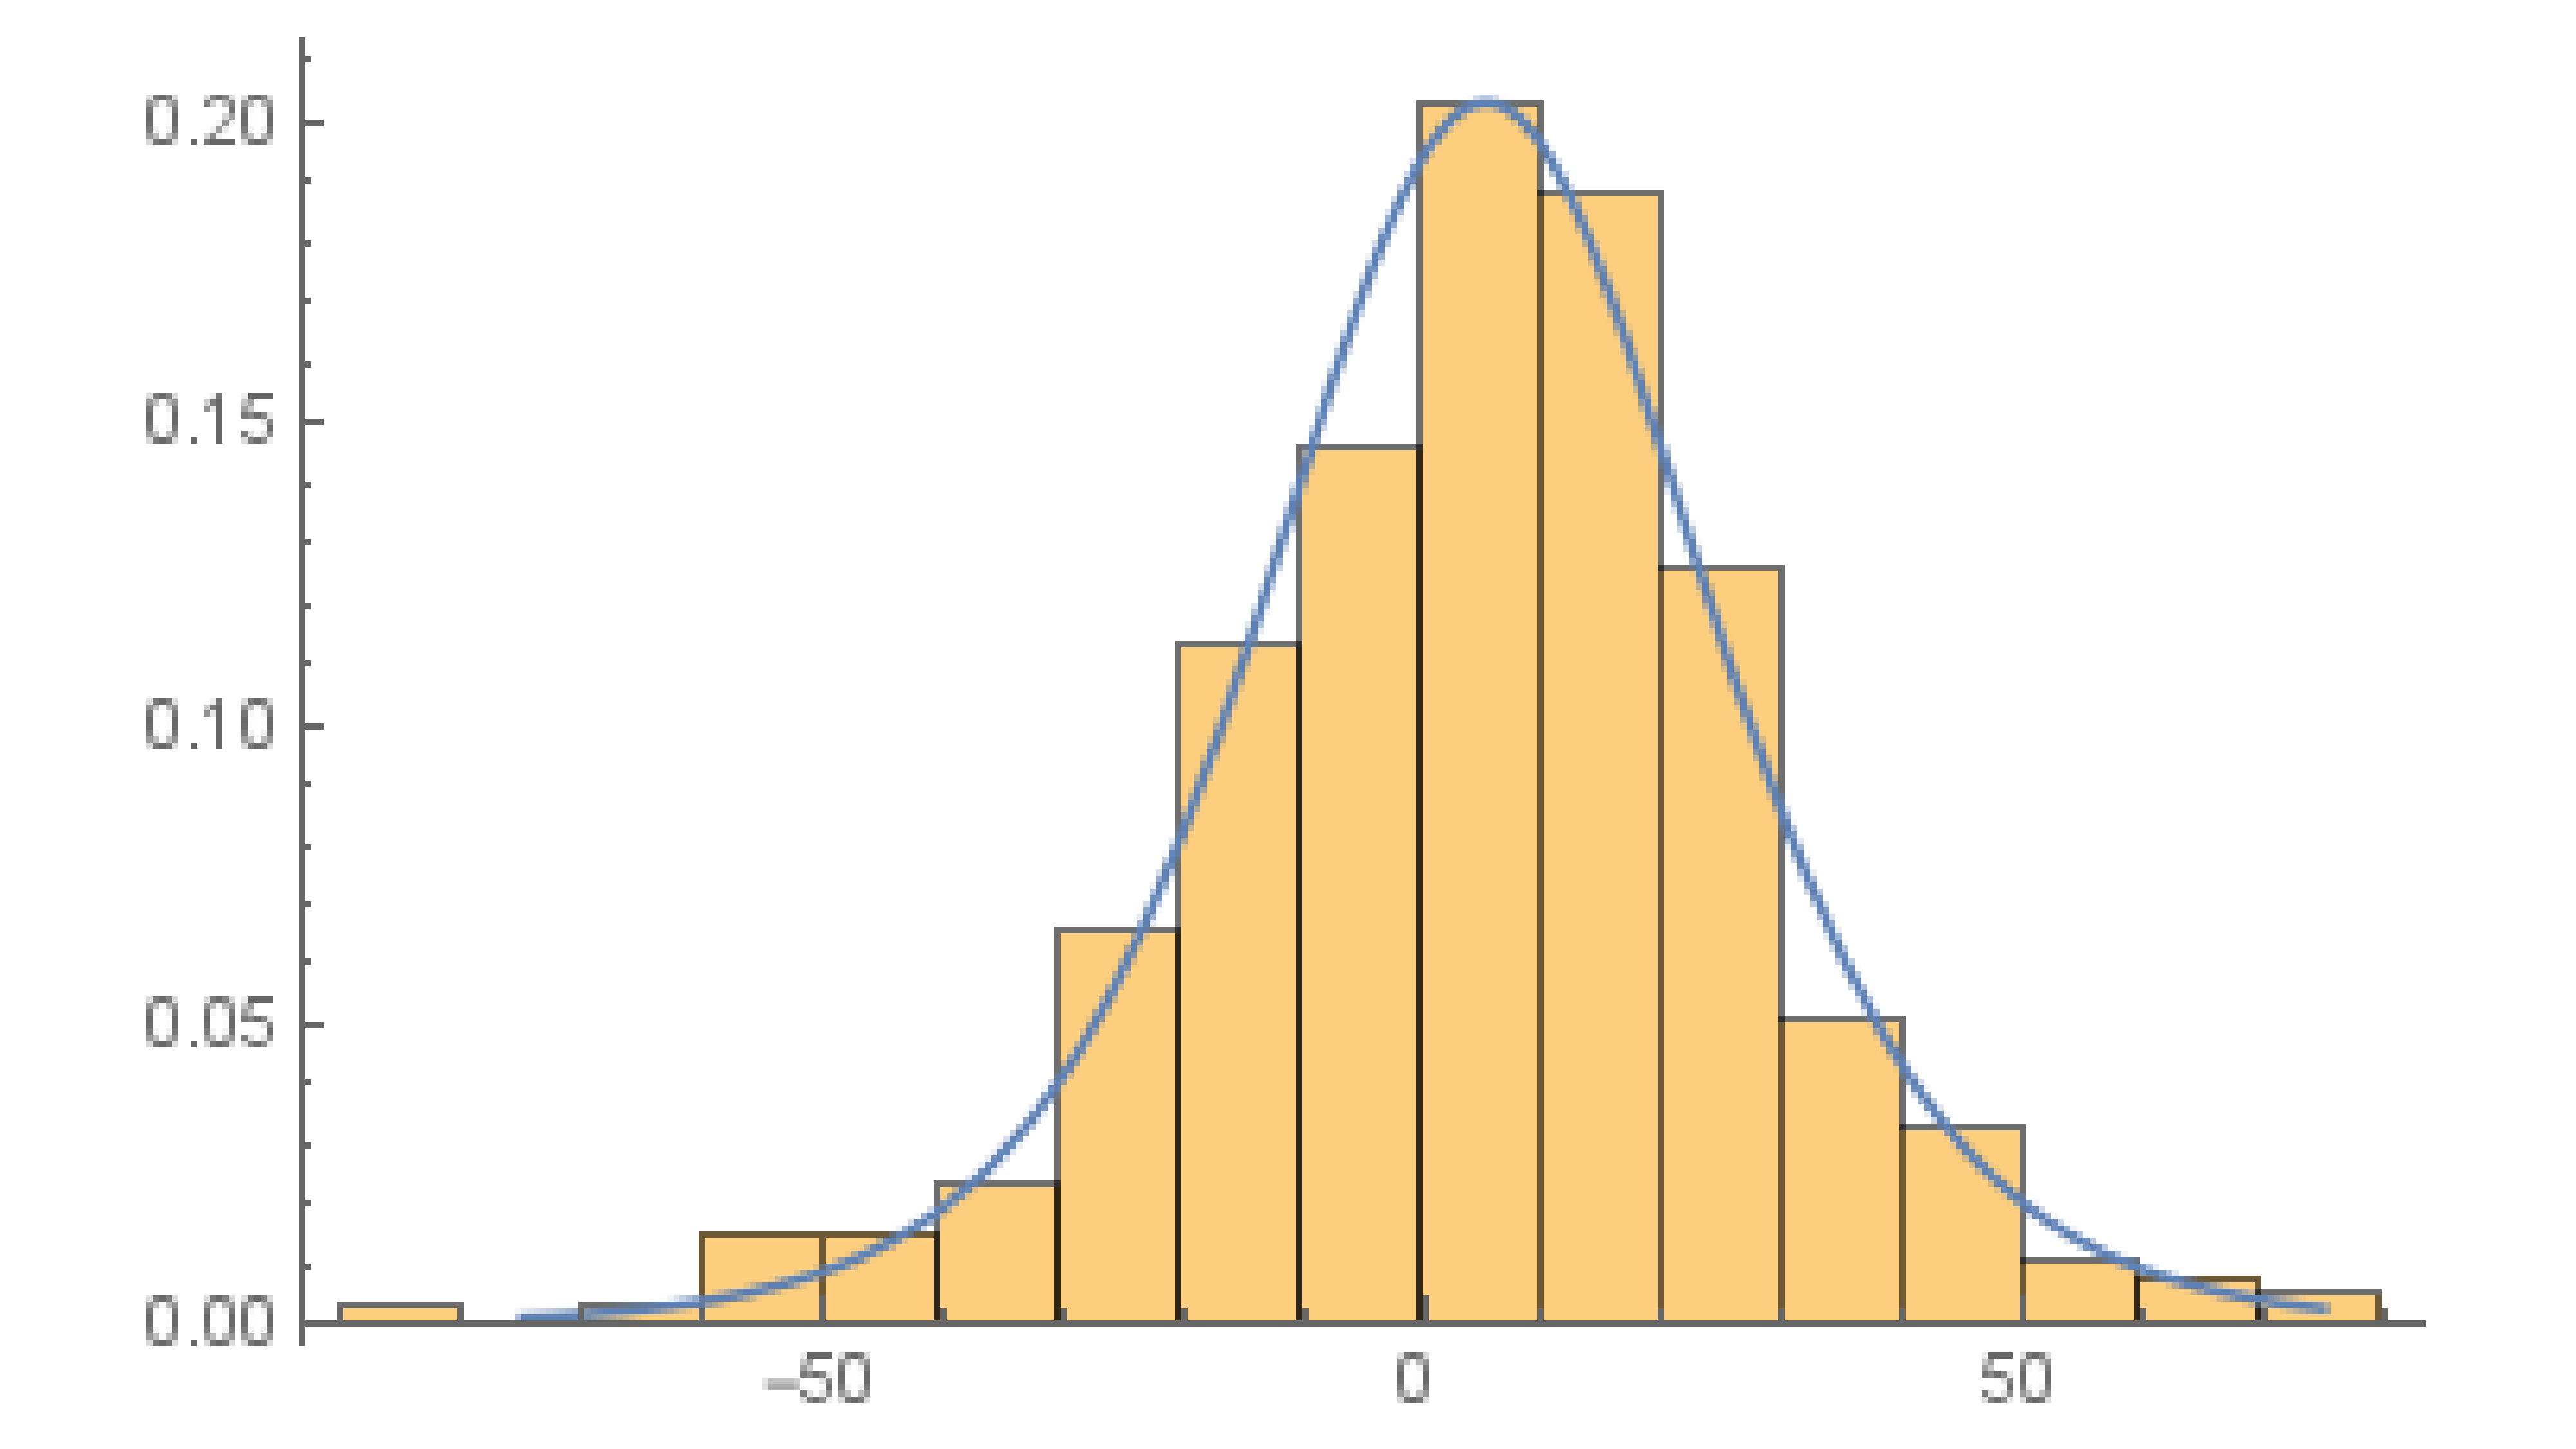
\includegraphics{log-histogram}
  \caption{Above is a normalized histogram of 
  differences between the values of the MWD GR and a well fitted 
  type log across 200 feet above the curve section. This probability distribution tells us,
  given a MWD GR reading, the probability that the underlying
  type log value is any certain value. In this case, if you read a
  value of 90 gAPI, there's about 20\% chance the underlying type log
  value is also 90, but a 1 or 2\% chance it's 40 or 140 gAPI. }
  \label{fig:log-histogram}
\end{marginfigure}

So at each of the wellbore positions in figure \ref{fig:random-vars-lateral}, we'll have a random variable for the MWD GR value. Before we take a measurement, we have some knowledge about it. We don't know what the measurement will be, but we know that whatever it turns out to be, it will be within a range of the true value for that stratum defined by the statistics we estimated above.   

Usually we don't have continuous inclination. We'll have inclination measurements every stand of pipe or so. But we'll define random variables for the inclinations at all the positions, initialize them using your prior estimates of inclination there, along with your confidence in those estimates, and then apply the evidence at those positions where we obtain surveys.

Now the wellbore inclination there; the dip of the geologic
structure 


The most important 

\section{Page Layout}\label{sec:page-layout}
\subsection{Headings}\label{sec:headings}
This style provides \textsc{a}- and \textsc{b}-heads (that is,
\Verb|\section| and \Verb|\subsection|), demonstrated above.

The Tufte-\LaTeX\ classes will emit an error if you try to use
\linebreak\Verb|\subsubsection| and smaller headings.

% let's start a new thought -- a new section
\newthought{In his later books},\cite{Tufte2006} Tufte
starts each section with a bit of vertical space, a non-indented paragraph,
and sets the first few words of the sentence in \textsc{small caps}.  To
accomplish this using this style, use the \Verb|\newthought| command:  
\begin{docspec}
  \doccmd{newthought\{In his later books\}, Tufte starts\ldots}
\end{docspec}

\subsection{Sidenotes}\label{sec:sidenotes}
One of the most prominent and distinctive features of this style is the
extensive use of sidenotes.  There is a wide margin to provide ample room
for sidenotes and small figures.  Any \Verb|\footnote|s will automatically
be converted to sidenotes.\footnote{This is a sidenote that was entered
using the \texttt{\textbackslash footnote} command.}  If you'd like to place ancillary
information in the margin without the sidenote mark (the superscript
number), you can use the \Verb|\marginnote| command.\marginnote{This is a
margin note.  Notice that there isn't a number preceding the note, and
there is no number in the main text where this note was written.}

The specification of the \Verb|\sidenote| command is:
\begin{docspec}
  \doccmd{sidenote[\docopt{number}][\docopt{offset}]\{\docarg{Sidenote text.}\}}
\end{docspec}

Both the \docopt{number} and \docopt{offset} arguments are optional.  If you
provide a \docopt{number} argument, then that number will be used as the
sidenote number.  It will change of the number of the current sidenote only and
will not affect the numbering sequence of subsequent sidenotes.

Sometimes a sidenote may run over the top of other text or graphics in the
margin space.  If this happens, you can adjust the vertical position of the
sidenote by providing a dimension in the \docopt{offset} argument.  Some
examples of valid dimensions are:
\begin{docspec}
  \ttfamily 1.0in \qquad 2.54cm \qquad 254mm \qquad 6\Verb|\baselineskip|
\end{docspec}
If the dimension is positive it will push the sidenote down the page; if the
dimension is negative, it will move the sidenote up the page.

While both the \docopt{number} and \docopt{offset} arguments are optional, they
must be provided in order.  To adjust the vertical position of the sidenote
while leaving the sidenote number alone, use the following syntax:
\begin{docspec}
  \doccmd{sidenote[][\docopt{offset}]\{\docarg{Sidenote text.}\}}
\end{docspec}
The empty brackets tell the \Verb|\sidenote| command to use the default
sidenote number.

If you \emph{only} want to change the sidenote number, however, you may
completely omit the \docopt{offset} argument:
\begin{docspec}
  \doccmd{sidenote[\docopt{number}]\{\docarg{Sidenote text.}\}}
\end{docspec}

The \Verb|\marginnote| command has a similar \docarg{offset} argument:
\begin{docspec}
  \doccmd{marginnote[\docopt{offset}]\{\docarg{Margin note text.}\}}
\end{docspec}

\subsection{References}
References are placed alongside their citations as sidenotes,
as well.  This can be accomplished using the normal \Verb|\cite|
command.\sidenote{The first paragraph of this document includes a citation.}

The complete list of references may also be printed automatically by using
the \Verb|\bibliography| command.  (See the end of this document for an
example.)  If you do not want to print a bibliography at the end of your
document, use the \Verb|\nobibliography| command in its place.  

To enter multiple citations at one location,\cite{Tufte2006,Tufte1990} you can
provide a list of keys separated by commas and the same optional vertical
offset argument: \Verb|\cite{Tufte2006,Tufte1990}|.  
\begin{docspec}
  \doccmd{cite[\docopt{offset}]\{\docarg{bibkey1,bibkey2,\ldots}\}}
\end{docspec}

\section{Figures and Tables}\label{sec:figures-and-tables}
Images and graphics play an integral role in Tufte's work.
In addition to the standard \docenv{figure} and \docenv{tabular} environments,
this style provides special figure and table environments for full-width
floats.

Full page--width figures and tables may be placed in \docenv{figure*} or
\docenv{table*} environments.  To place figures or tables in the margin,
use the \docenv{marginfigure} or \docenv{margintable} environments as follows
(see figure~\ref{fig:marginfig}):

\begin{marginfigure}%
  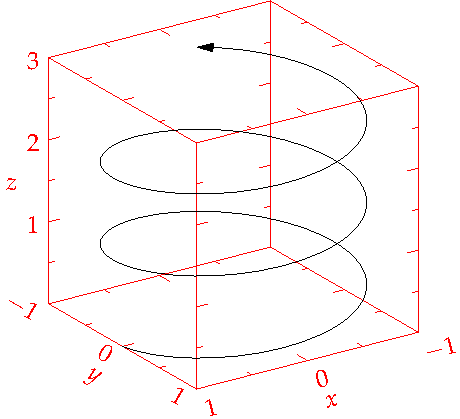
\includegraphics[width=\linewidth]{helix}
  \caption{This is a margin figure.  The helix is defined by 
    $x = \cos(2\pi z)$, $y = \sin(2\pi z)$, and $z = [0, 2.7]$.  The figure was
    drawn using Asymptote (\url{http://asymptote.sf.net/}).}
  \label{fig:marginfig}
\end{marginfigure}
\begin{Verbatim}
\begin{marginfigure}
  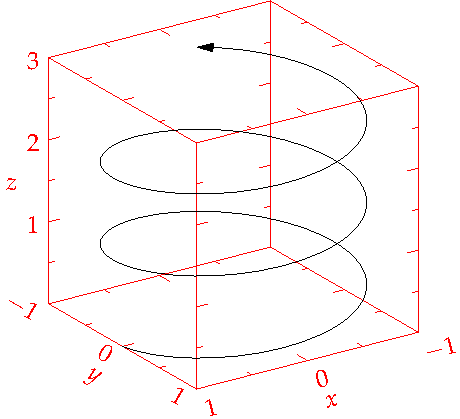
\includegraphics{helix}
  \caption{This is a margin figure.}
\end{marginfigure}
\end{Verbatim}

The \docenv{marginfigure} and \docenv{margintable} environments accept an optional parameter \docopt{offset} that adjusts the vertical position of the figure or table.  See the ``\nameref{sec:sidenotes}'' section above for examples.  The specifications are:
\begin{docspec}
  \doccmd{begin\{marginfigure\}[\docopt{offset}]}\\
  \qquad\ldots\\
  \doccmd{end\{marginfigure\}}\\
  \mbox{}\\
  \doccmd{begin\{margintable\}[\docopt{offset}]}\\
  \qquad\ldots\\
  \doccmd{end\{margintable\}}\\
\end{docspec}

Figure~\ref{fig:fullfig} is an example of the \Verb|figure*|
environment and figure~\ref{fig:textfig} is an example of the normal
\Verb|figure| environment.

\begin{figure*}[h]
  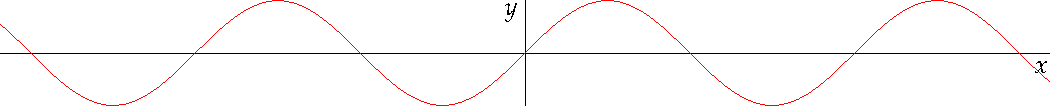
\includegraphics[width=\linewidth]{sine.pdf}%
  \caption{This graph shows $y = \sin x$ from about $x = [-10, 10]$.
  \emph{Notice that this figure takes up the full page width.}}%
  \label{fig:fullfig}%
\end{figure*}

\begin{figure}
  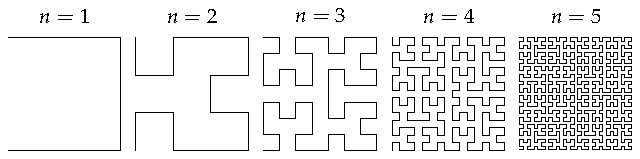
\includegraphics{hilbertcurves.pdf}
%  \checkparity This is an \pageparity\ page.%
  \caption{Hilbert curves of various degrees $n$.
  \emph{Notice that this figure only takes up the main textblock width.}}
  \label{fig:textfig}
  %\zsavepos{pos:textfig}
  \setfloatalignment{b}
\end{figure}

Table~\ref{tab:normaltab} shows table created with the \docpkg{booktabs}
package.  Notice the lack of vertical rules---they serve only to clutter
the table's data.

\begin{table}[ht]
  \centering
  \fontfamily{ppl}\selectfont
  \begin{tabular}{ll}
    \toprule
    Margin & Length \\
    \midrule
    Paper width & \unit[8\nicefrac{1}{2}]{inches} \\
    Paper height & \unit[11]{inches} \\
    Textblock width & \unit[6\nicefrac{1}{2}]{inches} \\
    Textblock/sidenote gutter & \unit[\nicefrac{3}{8}]{inches} \\
    Sidenote width & \unit[2]{inches} \\
    \bottomrule
  \end{tabular}
  \caption{Here are the dimensions of the various margins used in the Tufte-handout class.}
  \label{tab:normaltab}
  %\zsavepos{pos:normaltab}
\end{table}

\section{Full-width text blocks}

In addition to the new float types, there is a \docenv{fullwidth}
environment that stretches across the main text block and the sidenotes
area.

\begin{Verbatim}
\begin{fullwidth}
Lorem ipsum dolor sit amet...
\end{fullwidth}
\end{Verbatim}

\begin{fullwidth}
\small\itshape\lipsum[1]
\end{fullwidth}

\section{Typography}\label{sec:typography}

\subsection{Typefaces}\label{sec:typefaces}
If the Palatino, \textsf{Helvetica}, and \texttt{Bera Mono} typefaces are installed, this style
will use them automatically.  Otherwise, we'll fall back on the Computer Modern
typefaces.

\subsection{Letterspacing}\label{sec:letterspacing}
This document class includes two new commands and some improvements on
existing commands for letterspacing.

When setting strings of \allcaps{ALL CAPS} or \smallcaps{small caps}, the
letter\-spacing---that is, the spacing between the letters---should be
increased slightly.\cite{Bringhurst2005}  The \Verb|\allcaps| command has proper letterspacing for
strings of \allcaps{FULL CAPITAL LETTERS}, and the \Verb|\smallcaps| command
has letterspacing for \smallcaps{small capital letters}.  These commands
will also automatically convert the case of the text to upper- or
lowercase, respectively.

The \Verb|\textsc| command has also been redefined to include
letterspacing.  The case of the \Verb|\textsc| argument is left as is,
however.  This allows one to use both uppercase and lowercase letters:
\textsc{The Initial Letters Of The Words In This Sentence Are Capitalized.}



\section{Installation}\label{sec:installation}
To install the Tufte-\LaTeX\ classes, simply drop the
following files into the same directory as your \texttt{.tex}
file:
\begin{quote}
  \ttfamily
  tufte-common.def\\
  tufte-handout.cls\\
  tufte-book.cls
\end{quote}

% TODO add instructions for installing it globally



\section{More Documentation}\label{sec:more-doc}
For more documentation on the Tufte-\LaTeX{} document classes (including commands not
mentioned in this handout), please see the sample book.

\section{Support}\label{sec:support}

The website for the Tufte-\LaTeX\ packages is located at
\url{http://code.google.com/p/tufte-latex/}.  On our website, you'll find
links to our \smallcaps{svn} repository, mailing lists, bug tracker, and documentation.

\bibliography{sample-handout}
\bibliographystyle{plainnat}



\end{document}